\subsection{Independent Set (IS)}
Given a graph $G= (V, E)$, an independent set is a subset $S \subseteq V$ such that for any two vertices $u, v \in S$, there is no edge between $u$ and $v$.

The independent set decision problem (IS):
\begin{itemize}
	\item Instance: graph $G$ and number $K$
	\item Question: does $G$ have an independent set of size $K$?
\end{itemize}

Clearly, this is a NP problem. The certificate is just the $K$ vertices that form an independent set.

\subsection{Independent Set is NP-Compelete}

We show that 3-SAT reduces to Independent Set. 

\subsubsection{Main Idea}
The reduction maps literals into nodes of a graph, with the idea that a set of true literals will form an independent set.

\begin{itemize}
	\item Problem: in a YES-instance of 3-SAT, we can have one, two, or three literals true in each clause. So we do not get a definite size for the independent set.
	\item Solution: ensure that at most  one true literal in each clause can be part of the independent set, by connecting the 3 literals of the clause by a triangle.
\end{itemize}

Now, set the target size of the independent set to be $m$, the number of clauses. Only way to get to target is to pick exactly one literal from every clause. Since these literals have to be non-conflicting (to make an independent set), they can be simultaneously set to true, proving that the formula is satisfiable.

Let $\phi = \wedge_{i=1}^m C_i$, the $i$-th clause, is equal to $(\ell_1^i + \ell_2^i + \ell_3^i)$. The reduction $f$ transforms $\varphi$ into a graph $G$ and a number $K$ such that $\varphi$ is satisfiable if and only if $f(\varphi)$ is a YES-instance of Independent Set.

It seems mysterious that we can transform a logic problem into a graph problem. The main idea is to remember that to make $\varphi$ true, we must make at least 1 literal true in each clause. Also, rules of Boolean logic say we cannot choose to make $x$ true in one clause and $\bar{x}$ true in another; these are conflicting literals that cannot both be true.

Even though a satisfying assignment could make more than one literal true, we convert the clause into a triangle where an independent set can pick just one vertex. If two clauses have conflicting literals, we draw an edge between the corresponding nodes. Thus, an independent set can never pick nodes corresponding to conflicting literals. We now set $K = m$ and ask if $G$ has an independent set of size $K$.

\begin{figure}[H]
	\centering
	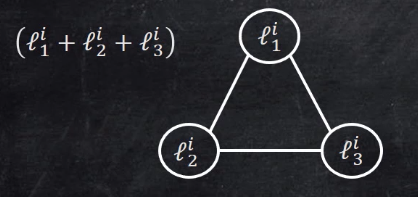
\includegraphics[width=0.3\textwidth]{fig/3-literal.png}	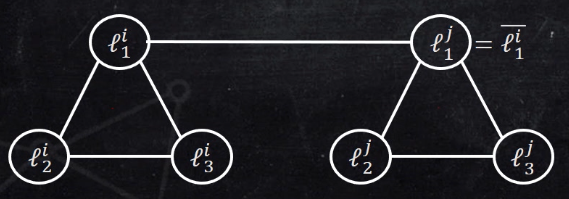
\includegraphics[width=0.4\textwidth]{fig/converse-literal.png}
\end{figure}

\subsubsection{Proof of Correctness}
If $\varphi$ is satisfiable:
\begin{itemize}
	\item In the satisfying assignment, we can find one literal per clause that is true.
	\item Since these literal are simultaneously true, there cannot be conflicting literals among them.
	\item In the graph, there are $m$ nodes corresponding to these literals, one per clause triangle.
	\item These $m$ nodes from an independent set (no edges due to conflicts), hence we have created a YES-instance of independent set.
\end{itemize}
 
Conversely, suppose $G$ is a YES-instance of IS:
\begin{itemize}
	\item Let $S$ be the subset of $m$ nodes that forms an independent set.
	\item Clearly, $S$ contains one node from each clause, and it contains no conflicting literals.
	\item Making all the literals corresponding to $S$ true causes $\varphi$ to be true.
	\item Thus we must have started with a YES-instance of 3-SAT.
\end{itemize}
 
\subsection{Points to Note}

To prove a reduction from $A$ to $B$ correct, we have to prove YES-instances of $A$ map to YES-instance of $B$ and NO-instances of $A$ map to NO-instances of $B$.

It is often convenient to do the second part by proving the equivalent contra-positive statement: \textbf{If the instance of $B$ created by the reduction is a YES-instance, it must have come from a YES-instance of $A$.}  
 
A reduction from $A$ to $B$ is a function whose domain is the instances of $A$. So it must be defined on ``all''  instances of $A$. However, it does not have to be one-to-one or onto, so not all instances of $B$ might be in the image of the reduction.
 
 
 
 
 
 
 
 
 
 
 
 
 
 
 
 
 
 
 
 